\chapter{Testing Stuff}
\section{SourceCode}
Hier ist wichtiger SourceCode. Es wäre toll wenn er so im Codeverzeichnis aufgeführt wird.
\begin{lstlisting}[caption=Test um SourceCode zu zeigen, label=codeExample]
main(){
    printf("Hello");
}
\end{lstlisting}

\section{Bild}
Ein jedes Bild sollte im Abbildungsverzeichnis gelistet sein.
\begin{figure}[ht]
    \centering
    
\includegraphics[width=\textwidth]{images/logoipsum.png}
    \caption{Das ist ein Logo}
    \label{fig:ExampleImage}
\end{figure}


\section{Tabelle}
Wenn man den Überblick über all seine tabellen verliert, passieren schlimme Dinge
\begin{table}[H]
    \centering
    \begin{tabular}{|c|c|}
        \hline
        HTTP Methode & boring \\
        \hline
    \end{tabular}
    \caption{Untertitel der Tabelle}
    \label{tab:Requests}
\end{table}

\section{Compilieren}
Um das gesamte Dokument mit Glossar und Literaturverzeichnis zu erstellen müssen die folgenden Befehle ausgeführt werden.

\begin{lstlisting}[caption=Compilieren des Dokuments, label=CompileInstructions]
pdflatex main           // Wird Sauer sein wegen fehlender Einträge. Mit "CTRL + C" Fehlermeldungen skippen

makeglossaries main     // Glossar generieren

pdflatex main           // Mit korrektem Glossar kann eine Hilfsdatei für Biber erstellt werden

biber main              // Biblatex Datei verarbeiten

pdflatex main           // Literaturverweise verwenden

pdflatex main           // Zweiter Durchlauf um Seitenzahlen zu korrigieren
\end{lstlisting}

\section{Citations}
Es ist unmöglich aus Vim zu entkommen \cite{nerd_how_2012}

\section{PlantUML}
Das Visal Studio Code Plugin bietet die Möglichkeit PUML Diagramme direkt zu \LaTeX zu exportieren.

\begin{figure}[H]
    \centering
    % generated by Plantuml 1.2024.3       
\definecolor{plantucolor0000}{RGB}{24,24,24}
\definecolor{plantucolor0001}{RGB}{0,0,0}
\definecolor{plantucolor0002}{RGB}{226,226,240}
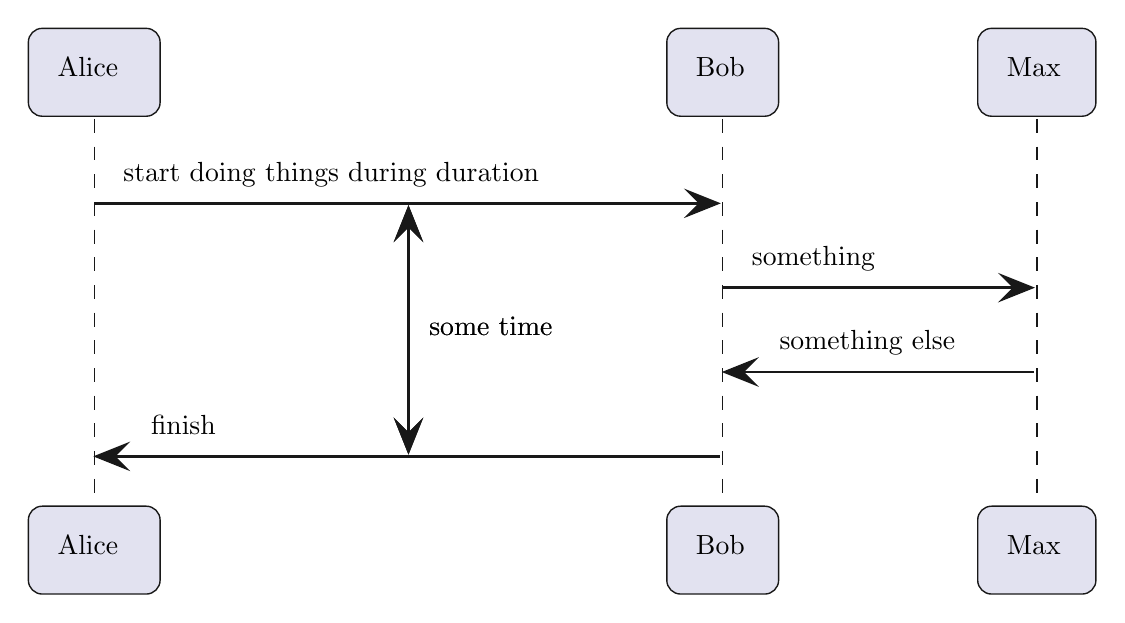
\begin{tikzpicture}[yscale=-1
,pstyle0/.style={color=plantucolor0000,line width=1.0pt}
,pstyle1/.style={color=plantucolor0000,fill=plantucolor0000,line width=1.0pt}
,pstyle2/.style={color=plantucolor0000,line width=0.5pt,dash pattern=on 5.0pt off 5.0pt}
,pstyle3/.style={color=plantucolor0000,fill=plantucolor0002,line width=0.5pt}
]
\draw[pstyle0] (142.3503pt,70.2246pt) -- (142.3503pt,157.6602pt);
\draw[pstyle1] (138.3503pt,80.2246pt) -- (142.3503pt,70.2246pt) -- (146.3503pt,80.2246pt) -- (142.3503pt,76.2246pt) -- cycle;
\draw[pstyle1] (138.3503pt,147.6602pt) -- (142.3503pt,157.6602pt) -- (146.3503pt,147.6602pt) -- (142.3503pt,151.6602pt) -- cycle;
\node at (146.3503pt,105.7031pt)[below right,color=black]{some time};
\draw[pstyle2] (28.8pt,37.7461pt) -- (28.8pt,177.6602pt);
\draw[pstyle2] (255.9006pt,37.7461pt) -- (255.9006pt,177.6602pt);
\draw[pstyle2] (369.4006pt,37.7461pt) -- (369.4006pt,177.6602pt);
\draw[pstyle3] (5pt,10pt) arc (180:270:5pt) -- (10pt,5pt) -- (47.6pt,5pt) arc (270:360:5pt) -- (52.6pt,10pt) -- (52.6pt,31.7461pt) arc (0:90:5pt) -- (47.6pt,36.7461pt) -- (10pt,36.7461pt) arc (90:180:5pt) -- (5pt,31.7461pt) -- cycle;
\node at (12pt,12pt)[below right,color=black]{Alice};
\draw[pstyle3] (235.7006pt,10pt) arc (180:270:5pt) -- (240.7006pt,5pt) -- (271.1006pt,5pt) arc (270:360:5pt) -- (276.1006pt,10pt) -- (276.1006pt,31.7461pt) arc (0:90:5pt) -- (271.1006pt,36.7461pt) -- (240.7006pt,36.7461pt) arc (90:180:5pt) -- (235.7006pt,31.7461pt) -- cycle;
\node at (242.7006pt,12pt)[below right,color=black]{Bob};
\draw[pstyle3] (348.0406pt,10pt) arc (180:270:5pt) -- (353.0406pt,5pt) -- (385.7606pt,5pt) arc (270:360:5pt) -- (390.7606pt,10pt) -- (390.7606pt,31.7461pt) arc (0:90:5pt) -- (385.7606pt,36.7461pt) -- (353.0406pt,36.7461pt) arc (90:180:5pt) -- (348.0406pt,31.7461pt) -- cycle;
\node at (355.0406pt,12pt)[below right,color=black]{Max};
\draw[pstyle3] (5pt,182.6602pt) arc (180:270:5pt) -- (10pt,177.6602pt) -- (47.6pt,177.6602pt) arc (270:360:5pt) -- (52.6pt,182.6602pt) -- (52.6pt,204.4063pt) arc (0:90:5pt) -- (47.6pt,209.4063pt) -- (10pt,209.4063pt) arc (90:180:5pt) -- (5pt,204.4063pt) -- cycle;
\node at (12pt,184.6602pt)[below right,color=black]{Alice};
\draw[pstyle3] (235.7006pt,182.6602pt) arc (180:270:5pt) -- (240.7006pt,177.6602pt) -- (271.1006pt,177.6602pt) arc (270:360:5pt) -- (276.1006pt,182.6602pt) -- (276.1006pt,204.4063pt) arc (0:90:5pt) -- (271.1006pt,209.4063pt) -- (240.7006pt,209.4063pt) arc (90:180:5pt) -- (235.7006pt,204.4063pt) -- cycle;
\node at (242.7006pt,184.6602pt)[below right,color=black]{Bob};
\draw[pstyle3] (348.0406pt,182.6602pt) arc (180:270:5pt) -- (353.0406pt,177.6602pt) -- (385.7606pt,177.6602pt) arc (270:360:5pt) -- (390.7606pt,182.6602pt) -- (390.7606pt,204.4063pt) arc (0:90:5pt) -- (385.7606pt,209.4063pt) -- (353.0406pt,209.4063pt) arc (90:180:5pt) -- (348.0406pt,204.4063pt) -- cycle;
\node at (355.0406pt,184.6602pt)[below right,color=black]{Max};
\draw[pstyle1] (243.9006pt,64.2246pt) -- (253.9006pt,68.2246pt) -- (243.9006pt,72.2246pt) -- (247.9006pt,68.2246pt) -- cycle;
\draw[pstyle0] (28.8pt,68.2246pt) -- (249.9006pt,68.2246pt);
\node at (35.8pt,49.7461pt)[below right,color=black]{start doing things during duration};
\draw[pstyle1] (357.4006pt,94.7031pt) -- (367.4006pt,98.7031pt) -- (357.4006pt,102.7031pt) -- (361.4006pt,98.7031pt) -- cycle;
\draw[pstyle0] (255.9006pt,98.7031pt) -- (363.4006pt,98.7031pt);
\node at (262.9006pt,80.2246pt)[below right,color=black]{something};
\draw[pstyle1] (266.9006pt,125.1816pt) -- (256.9006pt,129.1816pt) -- (266.9006pt,133.1816pt) -- (262.9006pt,129.1816pt) -- cycle;
\draw[pstyle0] (260.9006pt,129.1816pt) -- (368.4006pt,129.1816pt);
\node at (272.9006pt,110.7031pt)[below right,color=black]{something else};
\draw[pstyle1] (39.8pt,155.6602pt) -- (29.8pt,159.6602pt) -- (39.8pt,163.6602pt) -- (35.8pt,159.6602pt) -- cycle;
\draw[pstyle0] (33.8pt,159.6602pt) -- (254.9006pt,159.6602pt);
\node at (45.8pt,141.1816pt)[below right,color=black]{finish};
\draw[pstyle0] (142.3503pt,70.2246pt) -- (142.3503pt,157.6602pt);
\draw[pstyle1] (138.3503pt,80.2246pt) -- (142.3503pt,70.2246pt) -- (146.3503pt,80.2246pt) -- (142.3503pt,76.2246pt) -- cycle;
\draw[pstyle1] (138.3503pt,147.6602pt) -- (142.3503pt,157.6602pt) -- (146.3503pt,147.6602pt) -- (142.3503pt,151.6602pt) -- cycle;
\node at (146.3503pt,105.7031pt)[below right,color=black]{some time};
\end{tikzpicture}

    \caption{Das hier ist ein Diagram von PlantUml -> \LaTeX}
\end{figure}

Und noch ein zweites, diesmal aber mit einer veränderten Größe:
\begin{figure}[H]
    \centering
    \resizebox{10cm}{!}{
        % generated by Plantuml 1.2024.3       
\definecolor{plantucolor0000}{RGB}{24,24,24}
\definecolor{plantucolor0001}{RGB}{0,0,0}
\definecolor{plantucolor0002}{RGB}{226,226,240}
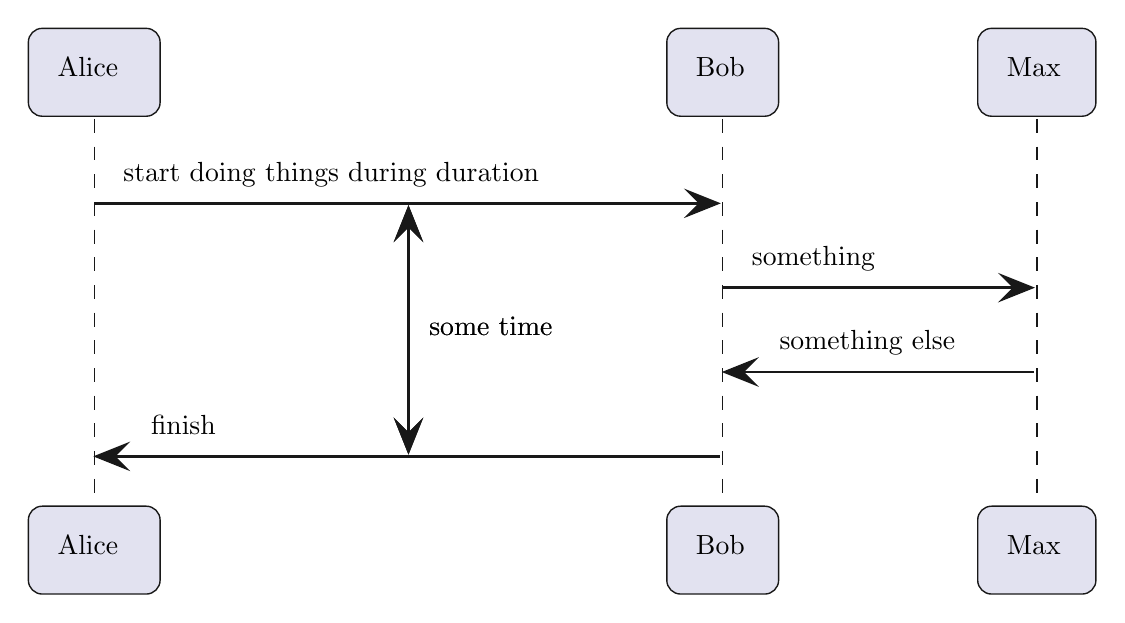
\begin{tikzpicture}[yscale=-1
,pstyle0/.style={color=plantucolor0000,line width=1.0pt}
,pstyle1/.style={color=plantucolor0000,fill=plantucolor0000,line width=1.0pt}
,pstyle2/.style={color=plantucolor0000,line width=0.5pt,dash pattern=on 5.0pt off 5.0pt}
,pstyle3/.style={color=plantucolor0000,fill=plantucolor0002,line width=0.5pt}
]
\draw[pstyle0] (142.3503pt,70.2246pt) -- (142.3503pt,157.6602pt);
\draw[pstyle1] (138.3503pt,80.2246pt) -- (142.3503pt,70.2246pt) -- (146.3503pt,80.2246pt) -- (142.3503pt,76.2246pt) -- cycle;
\draw[pstyle1] (138.3503pt,147.6602pt) -- (142.3503pt,157.6602pt) -- (146.3503pt,147.6602pt) -- (142.3503pt,151.6602pt) -- cycle;
\node at (146.3503pt,105.7031pt)[below right,color=black]{some time};
\draw[pstyle2] (28.8pt,37.7461pt) -- (28.8pt,177.6602pt);
\draw[pstyle2] (255.9006pt,37.7461pt) -- (255.9006pt,177.6602pt);
\draw[pstyle2] (369.4006pt,37.7461pt) -- (369.4006pt,177.6602pt);
\draw[pstyle3] (5pt,10pt) arc (180:270:5pt) -- (10pt,5pt) -- (47.6pt,5pt) arc (270:360:5pt) -- (52.6pt,10pt) -- (52.6pt,31.7461pt) arc (0:90:5pt) -- (47.6pt,36.7461pt) -- (10pt,36.7461pt) arc (90:180:5pt) -- (5pt,31.7461pt) -- cycle;
\node at (12pt,12pt)[below right,color=black]{Alice};
\draw[pstyle3] (235.7006pt,10pt) arc (180:270:5pt) -- (240.7006pt,5pt) -- (271.1006pt,5pt) arc (270:360:5pt) -- (276.1006pt,10pt) -- (276.1006pt,31.7461pt) arc (0:90:5pt) -- (271.1006pt,36.7461pt) -- (240.7006pt,36.7461pt) arc (90:180:5pt) -- (235.7006pt,31.7461pt) -- cycle;
\node at (242.7006pt,12pt)[below right,color=black]{Bob};
\draw[pstyle3] (348.0406pt,10pt) arc (180:270:5pt) -- (353.0406pt,5pt) -- (385.7606pt,5pt) arc (270:360:5pt) -- (390.7606pt,10pt) -- (390.7606pt,31.7461pt) arc (0:90:5pt) -- (385.7606pt,36.7461pt) -- (353.0406pt,36.7461pt) arc (90:180:5pt) -- (348.0406pt,31.7461pt) -- cycle;
\node at (355.0406pt,12pt)[below right,color=black]{Max};
\draw[pstyle3] (5pt,182.6602pt) arc (180:270:5pt) -- (10pt,177.6602pt) -- (47.6pt,177.6602pt) arc (270:360:5pt) -- (52.6pt,182.6602pt) -- (52.6pt,204.4063pt) arc (0:90:5pt) -- (47.6pt,209.4063pt) -- (10pt,209.4063pt) arc (90:180:5pt) -- (5pt,204.4063pt) -- cycle;
\node at (12pt,184.6602pt)[below right,color=black]{Alice};
\draw[pstyle3] (235.7006pt,182.6602pt) arc (180:270:5pt) -- (240.7006pt,177.6602pt) -- (271.1006pt,177.6602pt) arc (270:360:5pt) -- (276.1006pt,182.6602pt) -- (276.1006pt,204.4063pt) arc (0:90:5pt) -- (271.1006pt,209.4063pt) -- (240.7006pt,209.4063pt) arc (90:180:5pt) -- (235.7006pt,204.4063pt) -- cycle;
\node at (242.7006pt,184.6602pt)[below right,color=black]{Bob};
\draw[pstyle3] (348.0406pt,182.6602pt) arc (180:270:5pt) -- (353.0406pt,177.6602pt) -- (385.7606pt,177.6602pt) arc (270:360:5pt) -- (390.7606pt,182.6602pt) -- (390.7606pt,204.4063pt) arc (0:90:5pt) -- (385.7606pt,209.4063pt) -- (353.0406pt,209.4063pt) arc (90:180:5pt) -- (348.0406pt,204.4063pt) -- cycle;
\node at (355.0406pt,184.6602pt)[below right,color=black]{Max};
\draw[pstyle1] (243.9006pt,64.2246pt) -- (253.9006pt,68.2246pt) -- (243.9006pt,72.2246pt) -- (247.9006pt,68.2246pt) -- cycle;
\draw[pstyle0] (28.8pt,68.2246pt) -- (249.9006pt,68.2246pt);
\node at (35.8pt,49.7461pt)[below right,color=black]{start doing things during duration};
\draw[pstyle1] (357.4006pt,94.7031pt) -- (367.4006pt,98.7031pt) -- (357.4006pt,102.7031pt) -- (361.4006pt,98.7031pt) -- cycle;
\draw[pstyle0] (255.9006pt,98.7031pt) -- (363.4006pt,98.7031pt);
\node at (262.9006pt,80.2246pt)[below right,color=black]{something};
\draw[pstyle1] (266.9006pt,125.1816pt) -- (256.9006pt,129.1816pt) -- (266.9006pt,133.1816pt) -- (262.9006pt,129.1816pt) -- cycle;
\draw[pstyle0] (260.9006pt,129.1816pt) -- (368.4006pt,129.1816pt);
\node at (272.9006pt,110.7031pt)[below right,color=black]{something else};
\draw[pstyle1] (39.8pt,155.6602pt) -- (29.8pt,159.6602pt) -- (39.8pt,163.6602pt) -- (35.8pt,159.6602pt) -- cycle;
\draw[pstyle0] (33.8pt,159.6602pt) -- (254.9006pt,159.6602pt);
\node at (45.8pt,141.1816pt)[below right,color=black]{finish};
\draw[pstyle0] (142.3503pt,70.2246pt) -- (142.3503pt,157.6602pt);
\draw[pstyle1] (138.3503pt,80.2246pt) -- (142.3503pt,70.2246pt) -- (146.3503pt,80.2246pt) -- (142.3503pt,76.2246pt) -- cycle;
\draw[pstyle1] (138.3503pt,147.6602pt) -- (142.3503pt,157.6602pt) -- (146.3503pt,147.6602pt) -- (142.3503pt,151.6602pt) -- cycle;
\node at (146.3503pt,105.7031pt)[below right,color=black]{some time};
\end{tikzpicture}

    }
    \caption{Das hier ist ein weiteres Diagram von PlantUml -> \LaTeX}
\end{figure}